\section{Estimadores de actitud y de navegación}
\label{sec:estimadores}

\subsection{El problema que resuelven}

El giroscopio mide bien los cambios rápidos de actitud pero deriva: su
sesgo, integrado, crece sin límite. El acelerómetro y el magnetómetro dan
referencias absolutas (dirección de la gravedad y del norte magnético) pero
ruidosas, perturbables y, en el caso del acelerómetro de un multirrotor,
engañosas, como se verá enseguida. Un estimador de actitud (AHRS) fusiona
las tres fuentes. El simulador ofrece cuatro, intercambiables en caliente
(\cod{estimators.py}): \emph{ideal} (devuelve la verdad, sirve de línea
base), Madgwick, Mahony y un filtro de Kalman extendido. El estimador por
defecto es \val{estDef} (\cod{SimConfig.estimator}): con el acelerómetro
filtrado fue el más equilibrado entre escalones de actitud, maniobras y
seguimiento de trayectoria. Los tres reales comparten tres convenciones:
\begin{itemize}
\item la dirección de la gravedad medida en el cuerpo es
$\hat{\vect s}_g=-\vect a/\|\vect a\|$ (en reposo el acelerómetro lee
$(0,0,-g)$ en FRD);
\item trabajan en un NED magnético y rotan la salida por la declinación
(\cref{sec:marcos});
\item se inicializan con la primera muestra (\cod{triad\_alignment}): roll
y pitch del acelerómetro,
$\phi_0=\operatorname{atan2}(-a_y,-a_z)$,
$\theta_0=\operatorname{atan2}\big(a_x,\sqrt{a_y^2+a_z^2}\big)$, y rumbo del
magnetómetro compensado por inclinación,
$\psi_0=\operatorname{atan2}(-m_{h,y},m_{h,x})+D$, con
$m_{h,x}=m_x\cos\theta_0+m_y\sin\phi_0\sin\theta_0+m_z\cos\phi_0\sin\theta_0$ y
$m_{h,y}=m_y\cos\phi_0-m_z\sin\phi_0$.
\end{itemize}

\begin{nota}[Inicialización en el aire]
Si la simulación arranca en vuelo, la primera muestra trae la vibración de
las hélices (hasta 1.5~m/s$^2$) y alinear con ella dejaba errores iniciales
de varios grados ($\approx9^\circ$ de cabeceo medidos con Madgwick). Con
\cod{start\_airborne=True}, \cod{Simulation.\_prime\_airborne} inicializa el
estimador con la actitud verdadera. Es la hipótesis coherente con ``arrancar
en el aire'': el autopiloto real se alinea en tierra, con los motores
apagados, antes de despegar, y llega al vuelo con el estimador convergido.
Los sesgos y el ruido de los sensores se conservan; no es el estimador ideal.
\end{nota}

\subsection{El acelerómetro de un multirrotor no mide la gravedad}
\label{sec:leishman}

La \eqref{eq:fesp} dice que el acelerómetro mide
$\vect f_{acc}=(\vect f_B+\R\T\vect F_{ext})/m$: empuje más arrastre. En
vuelo estacionario inclinado $15^\circ$ y sin velocidad, el modelo da
$\vect f_{acc}=(0,\ 0,\ -9.80665)$, exactamente igual que nivelado: el roll
aparente que deduce el acelerómetro es $0^\circ$. Leishman, Macdonald, Beard
y McLain \cite{leishman14} lo explican con detalle: la idea de que el
acelerómetro ``mide la gravedad cuando no hay aceleración'' falla en un
multirrotor, porque inclinado \emph{siempre} acelera horizontalmente (salvo
que el arrastre lo equilibre), y lo que mide es la fuerza del rotor, alineada
con $z_B$.

La consecuencia práctica es que, durante una aceleración sostenida, un AHRS
que trate $-\vect a/\|\vect a\|$ como gravedad converge a ``nivelado'' y el
lazo de actitud, que cree estar en el ángulo pedido, sigue inclinando el
dron. El simulador implementa la corrección que usa PX4 (\cod{ATT\_ACC\_COMP}):
restar al acelerómetro la aceleración cinemática estimada por el filtro de
navegación antes de pasarlo al AHRS (\cod{SimConfig.acc\_compensation},
activa por defecto con el dron armado y, como se explica más abajo, solo
cuando el filtro de navegación recibe correcciones de posición absoluta). La
cadena completa del acelerómetro
hacia el AHRS (\cod{Simulation.step\_control}) es, por eje,
\begin{gather}
\vect a_{kin,E} = \operatorname{sat}_{0.8g}\Big(\mathcal{H}_{\val{accLpf}}\Big\{\frac{\hat{\vect v}_k-\hat{\vect v}_{k-1}}{\Delta t}\Big\}\Big),\label{eq:akin}\\
\vect a_{AHRS} = \mathcal{H}_{\val{accLpf}}\{\vect a_{med}\} - \kappa\,\hat\R\T\vect a_{kin,E},\qquad \kappa\in[0,1],\label{eq:acomp}
\end{gather}
con $\mathcal H_{\val{accLpf}}$ un Butterworth de segundo orden de
\val{accLpf}~Hz (\cod{SimConfig.ahrs\_accel\_lpf\_hz}; 0 lo desactiva), que
quita la vibración antes de la normalización $\vect a/\|\vect a\|$
(\cref{sec:rectificacion}). La derivada de la velocidad estimada pasa por el
\emph{mismo} Butterworth que el acelerómetro, para que las dos señales que se
restan lleguen con el mismo retardo, y su norma se recorta a $0.8g$. La
ganancia $\kappa$ de la compensación sube o baja en rampa en 0.5~s
(\cod{acc\_comp\_ramp\_s}), de modo que activarla o perderla en vuelo no
produce un salto. Todo esto vive en \cod{quadsim/estimation.py}, una sola
cadena que usan la simulación y los barridos de estimadores. La rotación que
aparece en \eqref{eq:acomp} es
la \emph{estimada}, $\hat\R$, y no la verdadera: el AHRS no conoce otra. La
edición anterior escribía el resultado como $\approx-g\,\R\T\eu$, y esa
lectura solo vale si $\vect a_{kin,E}$ es la aceleración real medida por una
vía independiente del acelerómetro y $\hat\R\approx\R$. En ese caso, con
$\vect f_{acc}=\R\T(\dot{\vect v}-g\eu)$,
\[
\vect a_{AHRS}\approx\R\T(\dot{\vect v}-g\eu)-\hat\R\T\dot{\vect v}\approx-g\,\R\T\eu ,
\]
y el AHRS recibe la dirección verdadera de la gravedad. El problema es de
dónde sale $\vect a_{kin,E}$. El filtro de navegación predice con el
\emph{mismo} acelerómetro rotado con la actitud estimada,
$\vect a_E=\hat\R\vect f_{acc}+g\eu$ (\cref{eq:nav}). Entre correcciones de
posición, entonces, $\vect a_{kin,E}\approx\hat\R\vect f_{acc}+g\eu$ y
\[
\vect a_{AHRS}\approx\vect f_{acc}-\hat\R\T\big(\hat\R\vect f_{acc}+g\eu\big)=-g\,\hat\R\T\eu :
\]
el AHRS recibe su propia estimación de la gravedad. La compensación es
\emph{autorreferente}. La información real de gravedad solo entra a través
del término de corrección del filtro de navegación, es decir, de las medidas
de posición. Sin sensor de posición (solo barómetro, que no corrige el plano
horizontal) roll y pitch dejan de ser observables, y con ellos el sesgo del
giroscopio. La revisión externa lo reprodujo con Mahony en 30~s de vuelo
estacionario, partiendo de una alineación perfecta: con sensor de posición y
compensación el error de inclinación fue 0.45$^\circ$; solo con barómetro y
compensación creció a 15.2$^\circ$ (unos 0.5$^\circ$/s) con 157~m de deriva
horizontal; solo con barómetro y sin compensación quedó en 1.4$^\circ$.

De ahí la regla que aplica el núcleo (\cod{AccelCompensation.wanted}): la
compensación actúa solo si hubo una corrección \emph{horizontal} de posición
absoluta en los últimos 0.2~s (\cod{acc\_comp\_fix\_timeout\_s}), si el dron
está armado y en el aire y si el filtro de navegación ya se asentó (tras
\cod{settle} o 1~s después de un reinicio). En tierra, recién armado, la
velocidad del navegador reiniciado producía una $\vect a_{kin,E}$ espuria de
1.6--2.8~m/s$^2$. Además, el filtro de navegación rechaza medidas de
posición atípicas: las que superan 5 desviaciones estándar de la innovación
predicha (\cod{nav\_gate\_sigma}) y, a la vez, se alejan más de 25~cm de la
predicción (\cod{gate\_min\_m}). El piso absoluto evita que una predicción
sesgada, por ejemplo por un rumbo estimado desviado, haga rechazar medidas
buenas una tras otra (\cref{sec:lectura_banco}). Sin correcciones de posición el AHRS recibe el
acelerómetro filtrado sin compensar, que se equivoca durante las
aceleraciones sostenidas pero no deriva: en el mismo vuelo estacionario de
30~s, solo con barómetro, el error de inclinación pasó de 15.2 a
1.46$^\circ$ (prueba \cod{test\_baro\_only\_hover\_keeps\_tilt\_estimate}). Es la situación del dron
real del proyecto (ESP32 con BMP180 y sin captura de movimiento), así que la
compensación, tal como está, no le sirve: haría falta estimar
$\vect a_{kin,E}$ por una vía independiente (por ejemplo, la segunda
derivada filtrada de una posición medida o la aceleración de referencia de
la trayectoria) o una arquitectura acoplada en la que el error de actitud sea
estado del filtro de navegación, como el EKF2 de PX4.

Hay un segundo límite, de sincronía. La versión anterior suavizaba
$\vect a_{kin,E}$ con un filtro de primer orden fijo de 50~ms, que no dependía
de \cod{ahrs\_accel\_lpf\_hz}, y la calculaba después del AHRS, de modo que se
usaba un periodo tarde; el desfase frente a la ruta del acelerómetro era de
65.6~ms. Con el mismo Butterworth en las dos ramas y el cálculo antes del
AHRS bajó a 17.0~ms. Lo que queda es el atraso propio de la velocidad del
navegador: la posición llega con 10~ms de retardo y se fusiona como si fuera
actual.

El filtrado suaviza la derivada de la velocidad
estimada, que es ruidosa; la misma $\vect a_{kin,E}$ se entrega a los
controladores de posición en \cod{NavState.acc}. El filtro de navegación,
en cambio, predice con el acelerómetro sin filtrar
(\cref{eq:nav}).

\begin{figure}[H]
\centering
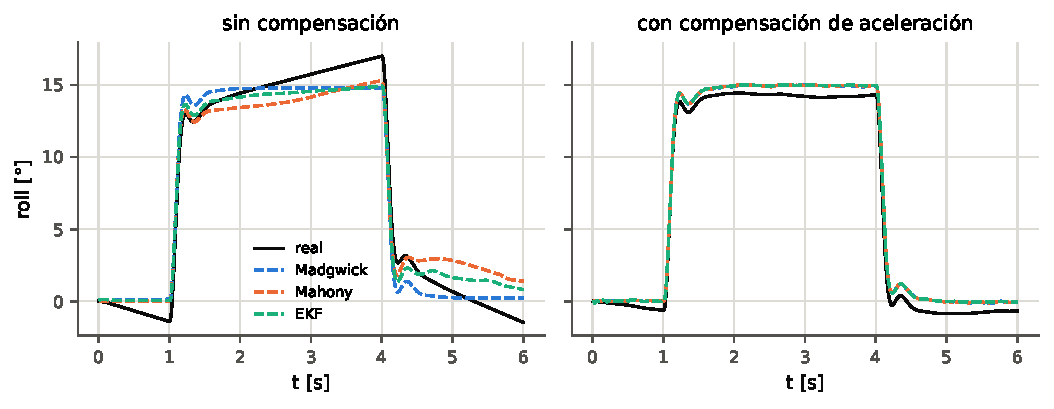
\includegraphics[width=\textwidth]{estimadores_aceleracion.pdf}
\caption{Roll real y estimado durante una inclinación sostenida de
$15^\circ$ (de $t=1$ a 4~s), sin y con compensación de aceleración.}
\label{fig:acc}
\end{figure}

La \cref{fig:acc} y la \cref{tab:acc} muestran el efecto. Sin compensación,
Mahony y el EKF ``ven'' 15$^\circ$ mientras el dron real llega a unos
31--34$^\circ$; con compensación el error máximo de los tres queda por debajo
de 1$^\circ$. Madgwick sin compensación se equivoca poco
(\val{mmadSe}$^\circ$) por una razón que no es mérito: con $\beta=\val{betaDef}$
su corrección por gravedad es tan lenta que en 3~s apenas se aparta de la
integración del giroscopio. Esa misma lentitud es la que lo atrasa en
maniobras largas.

\begin{table}[H]
\centering
\small
\caption{Inclinación sostenida de $15^\circ$ durante 3~s (bloque I):
error máximo del roll estimado y roll real al final del tramo.}
\label{tab:acc}
\begin{tabular}{lcccc}
\toprule
& \multicolumn{2}{c}{Sin compensación} & \multicolumn{2}{c}{Con compensación} \\
\cmidrule(lr){2-3}\cmidrule(lr){4-5}
Estimador & error máx [$^\circ$] & roll real [$^\circ$] & error máx [$^\circ$] & roll real [$^\circ$] \\
\midrule
Madgwick & \val{mmadSe} & \val{mmadSr} & \val{mmadCe} & \val{mmadCr} \\
Mahony   & \val{mmahSe} & \val{mmahSr} & \val{mmahCe} & \val{mmahCr} \\
EKF      & \val{mekfSe} & \val{mekfSr} & \val{mekfCe} & \val{mekfCr} \\
\bottomrule
\end{tabular}
\end{table}

\subsection{Madgwick}

Madgwick, Harrison y Vaidyanathan \cite{madgwick11} plantean la corrección
como un paso de descenso por gradiente sobre el error entre direcciones
medidas y predichas. Con $\vect d$ una dirección de referencia en $\E$ y
$\vect s$ su medida en $\B$, el residuo es $\vect f(\vect q)=\R(\vect q)\T\vect d-\vect s$
y su jacobiano analítico (\cod{\_jac\_rot\_inv}), con $\vect q=(w,\vect u)$:
\begin{equation}
\frac{\partial(\R\T\vect d)}{\partial w}=-2\,\vect u\times\vect d,\qquad
\frac{\partial(\R\T\vect d)}{\partial\vect u}=2w\,\sk{\vect d}+2\big((\vect u\cdot\vect d)I+\vect u\vect d\T-2\vect d\vect u\T\big).
\label{eq:jacmad}
\end{equation}
El código usa dos pares: gravedad, $\vect d_g=\eu$ con $\vect s=\hat{\vect s}_g$;
y campo magnético, $\vect d_m=\vect b$ con $\vect s=\hat{\vect m}$, donde la
referencia se reconstruye de la propia medida:
$\vect h=\R\hat{\vect m}$, $\vect b=(\sqrt{h_x^2+h_y^2},\,0,\,h_z)$. La
actualización (\cod{MadgwickEstimator.update}) es
\begin{equation}
\nabla=\sum_j J_j\T\vect f_j,\qquad
\dot{\vect q}=\tfrac12\vect q\otimes[0,\vect\omega_{med}]-\beta\,\frac{\nabla}{\|\nabla\|},\qquad
\vect q\leftarrow\frac{\vect q+\dot{\vect q}\,\Delta t}{\|\vect q+\dot{\vect q}\,\Delta t\|},
\label{eq:madgwick}
\end{equation}
con $\beta=\val{betaDef}$~rad/s por defecto. Dos rasgos importan al
interpretar resultados. El primero es que el paso de corrección está
\emph{normalizado}: su magnitud es siempre $\beta$, sea grande o pequeño el
error. Con un acelerómetro limpio (filtrado y compensado) el término
correctivo se comporta casi como un relé de amplitud $\beta$, y un $\beta$
grande produce un ciclo límite que el lazo de actitud amplifica. Se midió en
lazo cerrado con el núcleo actual: en la figura en 8
con el PID de posición, $\beta=0.1$ da 12.2~cm de RMSE, $\beta=0.03$ da
4.1~cm y $\beta=0.015$, 2.7~cm; en el escalón de roll, $\beta=0.12$ deja
2.5$^\circ$ de error de estimación. Por eso el valor por defecto es pequeño.
El precio es que, en maniobras sostenidas agresivas, el estimador se
atrasa. Este valor no coincide con el óptimo del barrido de $\beta$
(0.10--0.15, \cref{sec:barridos}): aquel barrido midió el error de
estimación \emph{en sombra} con la cadena de entonces, con el acelerómetro
crudo y sin realimentación del estimador sobre el vuelo, y el ciclo límite
solo aparece cuando el estimador cierra el lazo. El segundo rasgo es que esta implementación es la
versión sin compensación de deriva del giroscopio (el término $\zeta$ de la
sec.~3.4 del artículo no está): el sesgo no se estima y \cod{rates()}
entrega el giroscopio crudo.

\subsection{Mahony}

Mahony, Hamel y Pflimlin \cite{mahony08} formulan un filtro complementario
no lineal en $SO(3)$ con acción proporcional e integral. El error es el
producto cruz entre direcciones medidas y predichas:
\begin{equation}
\vect e=\hat{\vect s}_g\times(\R\T\eu)\ +\ \hat{\vect m}\times(\R\T\vect b),
\label{eq:mahony_e}
\end{equation}
con $\vect b$ construido como en Madgwick. La corrección y el integrador
(\cod{MahonyEstimator.update}):
\begin{equation}
\vect I\leftarrow\vect I+k_i\,\vect e\,\Delta t,\qquad
\hat{\vect b}_g=-\vect I,\qquad
\vect\omega_c=\vect\omega_{med}+k_p\vect e+\vect I,\qquad
\vect q\leftarrow\operatorname{norm}\!\big(\vect q+\tfrac12\vect q\otimes[0,\vect\omega_c]\Delta t\big),
\label{eq:mahony}
\end{equation}
con $k_p=\val{mahKp}$~rad/s y $k_i=\val{mahKi}$~rad/s$^2$ por defecto. El
integrador es exactamente el sesgo estimado del giroscopio, con el signo
cambiado, y se recorta al mismo tope que usa el EKF para el sesgo.

\paragraph{Magnetómetro solo para el rumbo.} Tal como están escritas,
\eqref{eq:madgwick} y \eqref{eq:mahony_e} dejan que el magnetómetro corrija
los tres ejes. Con una interferencia fuerte, que tiene componente vertical,
eso inclina también roll y pitch. En Madgwick y Mahony el código proyecta la
corrección magnética sobre el eje vertical terrestre expresado en el
cuerpo, como hace el estimador de actitud de PX4
(\cod{attitude\_estimator\_q}), de modo que el magnetómetro solo mueve el
rumbo. En el escenario \cod{estimator\_accuracy} con 40~$\mu$T de EMI, el
error de inclinación de Mahony bajó de 9.67 a 1.59$^\circ$ RMS y el de
Madgwick de 2.9 a 1.1$^\circ$; sin EMI la proyección cuesta unos
0.03$^\circ$, porque el campo correcto también aportaba algo de información
de inclinación. El EKF no lleva esta proyección.

\subsection{Filtro de Kalman extendido (7 estados)}

El EKF (\cod{EKFEstimator}) usa el estado $\vect x=[\vect q\T,\vect b_g\T]\T$
con formulación aditiva sobre el cuaternión y renormalización, en la línea
de Sabatini \cite{sabatini06}.

\paragraph{Predicción.} Con $\vect\omega=\vect\omega_{med}-\vect b_g$,
\begin{gather}
\bar{\vect q}=\operatorname{norm}\big(\vect q+\Omega(\vect\omega)\vect q\,\Delta t\big),\qquad
\Omega(\vect\omega)=\frac12\begin{bmatrix}0&-\omega_x&-\omega_y&-\omega_z\\
\omega_x&0&\omega_z&-\omega_y\\ \omega_y&-\omega_z&0&\omega_x\\ \omega_z&\omega_y&-\omega_x&0\end{bmatrix},\\
F=\begin{bmatrix}I_4+\Omega\Delta t & -\Xi(\vect q)\Delta t\\ 0 & I_3\end{bmatrix},\qquad
\Xi(\vect q)=\frac12\begin{bmatrix}-q_x&-q_y&-q_z\\ q_w&-q_z&q_y\\ q_z&q_w&-q_x\\ -q_y&q_x&q_w\end{bmatrix},\\
P\leftarrow FPF\T+Q,\qquad Q=\diag\big(\sigma_g^2\Delta t^2\,\Xi\Xi\T,\ \ \sigma_{bw}^2\Delta t\,I_3\big),
\end{gather}
con $\sigma_g=\val{ekfGyro}$~rad/s y $\sigma_{bw}=\val{ekfBias}$~rad/s/$\sqrt{\text{s}}$
por defecto, y $P_0=\diag(10^{-3}I_4,\,10^{-4}I_3)$.

\paragraph{Corrección.} Medidas: la dirección de la gravedad en cada paso, y
la dirección del campo magnético solo cuando hay muestra nueva (100~Hz). A
diferencia de Madgwick y Mahony, la referencia magnética es fija y conocida,
$\vect m_{ref}=(\cos I,0,\sin I)$ en el NED magnético:
\begin{gather}
\vect z=\begin{bmatrix}\hat{\vect s}_g\\ \hat{\vect m}\end{bmatrix},\quad
\vect h(\bar{\vect q})=\begin{bmatrix}\R\T\eu\\ \R\T\vect m_{ref}\end{bmatrix},\quad
H=\begin{bmatrix}J(\bar{\vect q},\eu) & 0\\ J(\bar{\vect q},\vect m_{ref}) & 0\end{bmatrix},\\
R=\diag\big(\sigma_a^2\,(1+k_{ad}\,\big|\|\vect a\|-g\big|/g)^2\,I_3,\ \ \sigma_m^2I_3\big),\\
K=PH\T(HPH\T+R)^{-1},\quad \vect x\leftarrow\vect x+K(\vect z-\vect h),\quad
P\leftarrow\tfrac12\big[(I-KH)P+((I-KH)P)\T\big],
\end{gather}
con $J$ de \eqref{eq:jacmad}, $\sigma_a=\val{ekfAcc}$, $\sigma_m=\val{ekfMag}$
(adimensionales: son ruidos sobre direcciones unitarias) y $k_{ad}=4$. Los
valores de $\sigma_a$ y $\sigma_m$ son los que el barrido de la
\cref{sec:barridos} encontró robustos frente a interferencia magnética; los
primeros valores del núcleo (0.05 y 0.05) confiaban demasiado en un
acelerómetro que la vibración desvía en $1.5/9.8\approx0.15$ de dirección, y
demasiado poco en la medida magnética. El factor adaptativo infla la covarianza del acelerómetro cuando su norma se
aleja de $g$, es decir, en maniobra. Tras la corrección se renormaliza el
cuaternión y el sesgo se acota a $\pm0.2$~rad/s.

\subsection{Resultados en vuelo estacionario}

La \cref{tab:hover_est} resume 10~s de vuelo estacionario en modo actitud
(después de 2~s de asentamiento), con y sin vibración.

\begin{table}[H]
\centering
\small
\caption{Error del estimador en hover, media / desviación estándar
[$^\circ$] (bloque I, semilla 1).}
\label{tab:hover_est}
\begin{tabular}{llccc}
\toprule
Estimador & Vibración & roll & pitch & yaw \\
\midrule
Madgwick & sí & \val{hmadVr} & \val{hmadVp} & \val{hmadVy} \\
         & no & \val{hmadNr} & \val{hmadNp} & \val{hmadNy} \\
Mahony   & sí & \val{hmahVr} & \val{hmahVp} & \val{hmahVy} \\
         & no & \val{hmahNr} & \val{hmahNp} & \val{hmahNy} \\
EKF      & sí & \val{hekfVr} & \val{hekfVp} & \val{hekfVy} \\
         & no & \val{hekfNr} & \val{hekfNp} & \val{hekfNy} \\
\bottomrule
\end{tabular}
\end{table}

Con el núcleo actual los tres estimadores quedan por debajo de
$0.65^\circ$ de error medio y de $0.15^\circ$ de desviación, y los resultados
con y sin vibración son prácticamente iguales: el pasa-bajos del
acelerómetro y el filtro del giroscopio la retiran. El error medio que queda
(0.5--0.6$^\circ$ en roll) es un sesgo lento, del orden de los
$0.3^\circ$ del sesgo inicial del acelerómetro ($0.05/9.8$~rad) más el resto
de la rectificación. Con el núcleo anterior el cuadro era otro: Madgwick
deambulaba con 1--2$^\circ$ de desviación y el EKF con vibración llegaba a
$1.6^\circ$; el paso normalizado de Madgwick con $\beta=0.08$ y el
$\sigma_a=0.05$ del EKF explicaban la diferencia.

\paragraph{Sesgo por rectificación de la vibración.}
\phantomsection\label{sec:rectificacion}
Esta es la razón del pasa-bajos de \eqref{eq:acomp}. La normalización
$\vect a/\|\vect a\|$ es no lineal: si la vibración $\vect n$ de cada rotor
actúa a lo largo de una dirección fija con componentes vertical y horizontal,
el término de segundo orden $-(\vect n\cdot\hat{\vect g})\vect n_\perp/g^2$
tiene media no nula, del orden de $A_a^2/(4g^2)\approx0.34^\circ$ por rotor.
El bloque I2 lo mide desactivando el filtro
(\cod{ahrs\_accel\_lpf\_hz = 0}): el error medio de inclinación (4 semillas,
5~s en hover) es \val{rectmadC}$^\circ$ con Madgwick, \val{rectmahC}$^\circ$
con Mahony y \val{rectekfC}$^\circ$ con el EKF. Con el Butterworth de
\val{accLpf}~Hz del núcleo (el equivalente de \cod{IMU\_ACCEL\_CUTOFF} de
PX4) baja a \val{rectmadF}, \val{rectmahF} y \val{rectekfF}$^\circ$. La
verificación de la 3.ª edición detectó este sesgo y el filtro se incorporó
al núcleo a raíz de ello.

\subsection{Filtro de navegación}

Los controladores de posición necesitan posición y velocidad estimadas.
\cod{NavEstimator} es un Kalman lineal independiente por eje con estado
$[p,v]$, el esqueleto lineal del EKF2 de PX4. Predice con la aceleración
medida llevada al marco inercial con la actitud \emph{estimada},
\begin{equation}
\vect a_E=\hat\R\,\vect a_{med}+g\eu,\qquad
\begin{bmatrix}p\\v\end{bmatrix}_{k+1}=\begin{bmatrix}1&\Delta t\\0&1\end{bmatrix}\begin{bmatrix}p\\v\end{bmatrix}_k+\begin{bmatrix}\Delta t^2/2\\ \Delta t\end{bmatrix}a_E,\qquad
P\leftarrow FPF\T+G\,q_a^2\,G\T,
\label{eq:nav}
\end{equation}
con $q_a=0.5$~m/s$^2$ (\cod{SimConfig.nav\_accel\_noise}, un valor de
diseño que cubre sobre todo la vibración y el error de actitud, no el ruido
blanco del acelerómetro), y corrige con el sensor de posición externo
($\sigma=0.01$~m, tres ejes) cuando llega una muestra nueva o, si no, con
el barómetro ($\sigma=0.17$~m, solo $z$). Un error de actitud de
$\delta$ radianes inyecta $g\,\delta$ de aceleración horizontal falsa en la
predicción: el estimador de navegación hereda los errores del AHRS, y esa
es una de las razones por las que el error de seguimiento depende del
estimador de actitud (\cref{sec:posicion}).

\begin{nota}[Detalles de implementación del filtro de navegación]
\begin{itemize}[leftmargin=1.2em]
\item El barómetro se fusiona aunque el sensor de posición esté activo: la
condición es \emph{posición nueva} o, en su defecto, \emph{barómetro nuevo},
y como las dos tasas no están sincronizadas, en 10~s se registraron
\val{navPos} correcciones de posición y \val{navBaro} de barómetro. El efecto
es despreciable porque $\sigma_{baro}\gg\sigma_{pos}$: el error RMS de la
altura estimada en 60~s es \val{zBaro}~mm con esa fusión y \val{zNoBaro}~mm
sin ella.
\item \cod{reset} deja $P=0.1\,I$; con esa covarianza inicial la ganancia
sobre la velocidad es grande durante unos 0.5~s y la velocidad estimada
tiene 5--8~cm/s de ruido. En un arranque en el aire,
\cod{NavEstimator.settle} itera el propio filtro durante 2~s con la medida
exacta y lleva $P$ a régimen sin cambiar el estado.
\end{itemize}
\end{nota}
